%%%%%%%%%%%% Attribution %%%%%%%%%%%%
% This template was created by 
% Chuck F. Rocca at WCSU and may be
% copied and used freely for 
% non-commercial purposes.
% 10-17-2021
%%%%%%%%%%%%%%%%%%%%%%%%%%%%%%%%%%%%%

%%%%%%% Start Document Header %%%%%%%
% In creating a new document
% copy and paste the header 
% as is.
%%%%%%%%%%%%%%%%%%%%%%%%%%%%%%%%%%%%%

\documentclass[12pt]{article}

%%%% Header Information %%%%
    %%% Document Settings %%%%
    \usepackage[utf8]{inputenc}
    \usepackage[
        twoside,
        top=1in,
        bottom=0.75in,
        inner=0.5in,
        outer=0.5in
    ]{geometry}
    \pagestyle{myheadings}

%%%% Additional Commands to Load %%%%
    \usepackage{tcolorbox}
    \tcbuselibrary{skins}
    \usepackage{minted}
    \usepackage{color}
    \usepackage{tikz}
    \usetikzlibrary{calc}
    \usepackage{tabularx,colortbl}
    \usepackage{amsfonts,amsmath,amssymb}
    \usepackage{titling}
    \usepackage{mathrsfs}
    \usepackage{calc}
    \usepackage{xepersian}

%%%% Commands to Define Homework Boxes %%%%
%%%% Box Definition %%%%
    \newtcolorbox{prob}[1]{
    % Set box style
        sidebyside,
        sidebyside align=bottom,
    % Dimensions and layout
        width=\textwidth,
        toptitle=2.5pt,
        bottomtitle=2.5pt,
        righthand width=0\textwidth,
    % Coloring
        colbacktitle=gray!30,
        coltitle=black,
        colback=white,
        colframe=white,
    % Title formatting
        title={
            #1 \hfill نمره:\phantom{WWWW}
        },
        fonttitle=\large\bfseries
    }

%%%% Environment Definition %%%%
    \newenvironment{problem}[1]{
        \begin{prob}{#1}
    }
    {
        \tcblower
        \centering
        \vspace{\baselineskip}
        \end{prob}
    }



%%%% Document Information %%%%
    \title{تمرین سری چهارم کنترل دیجیتال}
    \date{نیسمال دوم 1402-1403}
    \author{استاد درس : دکتر طالبی}

%%%%%%% End Document Header %%%%%%%


%%%% Begin Document %%%%
% note that the document starts with
% \begin{document} and ends with
% \end{document}
%%%%%%%%%%%%%%%%%%%%%%%%
\settextfont{BNAZANIN.TTF}

\begin{document}

%%%% Format Running Header %%%%%
\markboth{\theauthor}{\thetitle}

%%%% Insert the Title Information %%%
% \maketitle


%%%% General Description of the Document %%%%
\begin{figure}[htbp]
    \centering
    
\includegraphics[width=\linewidth]{Header.png}
    % \caption{Caption}
    % \label{fig:enter-label}
\end{figure}


%%%% Introduction to the General Template %%%%

    \begin{problem}{سوال اول}
    	(تست ژوری) با استفاده از تست ژوری پایداری سیستم زیر را بررسی کنید.
    	
    	\centering
    	$D(z) = z^3 -1.1z^2 - 0.1z + 0.3$
    	

    \end{problem}
    
    \begin{problem}{سوال دوم}
    	(تست ژوری)با استفاده از تست ژوری تعیین کنید سیستمی با معادله مشخصه زیر پایدار است یا خیر. تعداد ریشه های احتمالی خارج دایره واحده را تعیین کنید.
    	
    	\centering
    	$D(z) = z^3 - 2.2z^2 + 1.55z - 0.35$
 
    \end{problem}
    
    \begin{problem}{سوال سوم}
    	(مکان ریشه گسسته) نمودار مکان ریشه مربوط به شکل را رسم کنید.
    	
    	\lr{T = 2s}
    	
    	(امیتازی) نمودار رسم شده را مجدداً در متلب رسم کنید و با نتیجه خود مقایسه کنید
   
    \end{problem}
    \begin{figure}
    	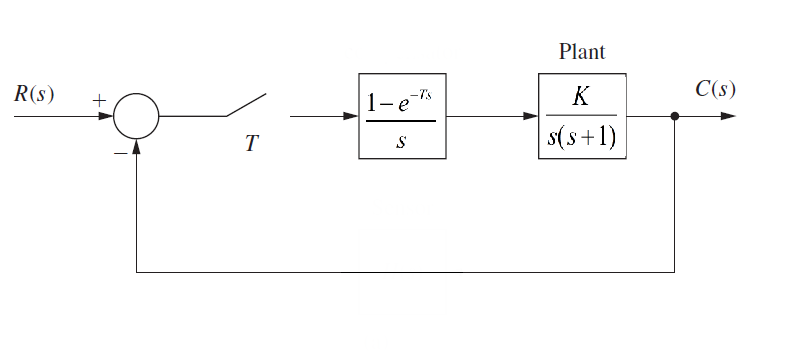
\includegraphics[width=\linewidth]{Resources/1.png}
    	\caption{شکل سوال سوم}
    \end{figure}
    
    \begin{problem}{سوال چهارم}
    	(ترکیبی (طراحی کنترلر + گسسته سازی + مکان ریشه گسسته)) الف) تابع تبدیل زیر را در نظر بگیرید. 
    	
    	\centering
    	$G(s) = \frac{K(s-2)}{s(s+1)}$
    	
    	\raggedright
    	کنترلری طراحی کنید که شرایط مقابل را برآورده سازد : 
    	$\omega_b = 1 rad/s$
    	,
    	$\phi_{pm} = 45$
    	
    	ب) کنترلر طراحی شده را به روش تطبیق قطب و صفر گسسته سازی کنید
    	
    	ج) با رسم مکان هندسی ریشه ها بررسی کنید که آیا مشخصات عملکردی برآورده شده است یا خیر.
    	
    	د) (امتیازی) نتایح بدست آمده را در متلب شبیه سازی کنید.
    \end{problem}
    
    \begin{problem}{سوال پنجم}
    	(تست ژوری) با استفاده از تست ژوری در مورد پایداری معادله مشخصه زیر و پایداری سیستم مربوطه بحث کنید.
    	
    	\centering
    	$D(z) = z^3 + (0.05K-1.2)z^2 + (0.07K + 0.2)z + (0.005K - 0.007)K$
    \end{problem}
    
    \begin{problem}{سوال ششم}
    	(برنامه ریزی) آیا مجموعه \lr{task} های زیر با روش 
    	\lr{Rate Monotonic (RM)}
    	قابل برنامه ریزی می باشد؟
    	
    	\centering
    	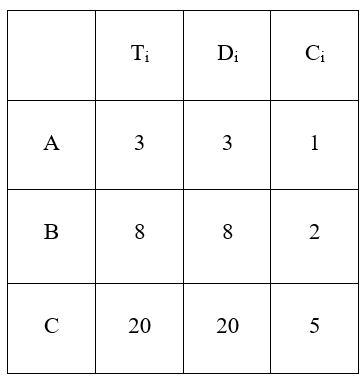
\includegraphics[scale=1]{Resources/2.png}
    \end{problem}


\end{document}
